

\documentclass[11pt]{exam}
\RequirePackage{amssymb, amsfonts, amsmath, latexsym, verbatim, xspace, setspace}
\usepackage{graphicx}

% By default LaTeX uses large margins.  This doesn't work well on exams; problems
% end up in the "middle" of the page, reducing the amount of space for students
% to work on them.
\usepackage[margin=1in]{geometry}
%\usepackage{Definitions}
\usepackage{tikz}
\usepackage{booktabs}
\usepackage{graphicx}
\usepackage{todonotes}
\usepackage{xcolor}
\usepackage{hyperref}

\hypersetup{colorlinks=true,linkcolor=blue,urlcolor=blue}

\setlength{\marginparwidth}{2.2cm}

\usepackage[shortlabels]{enumitem}
\setenumerate{label={\alph*)}}

% Here's where you edit the Class, Exam, Date, etc.
\newcommand{\class}{ Modeling Evolution Homework 3}
\newcommand{\term}{Spring 2025}
\newcommand{\examnum}{ Homework3}
\newcommand{\examdate}{ Spring 2025}




\DeclareMathOperator{\dom}{dom}
\newcommand{\norm}[1]{\lVert #1 \rVert}
\newcommand{\abs}[1]{\lvert #1 \rvert}
\newcommand{\st}{\mathrm{s.t.}}

% For an exam, single spacing is most appropriate
\singlespacing
% \onehalfspacing
% \doublespacing

% For an exam, we generally want to turn off paragraph indentation
\parindent 0ex

% It's nice to have big, section-style question headings
\usepackage{etoolbox}
\makeatletter
\patchcmd{\questions}
  {\def\@currentlabel{\thequestiontitle}}
  {\def\@currentlabel{\thequestion}}
  {}
  {}
\makeatother
\def\qstrut{\protect\rule[-3ex]{0ex}{3ex}} 
\qformat{\Large \textbf{\thequestion. \thequestiontitle~~(\totalpoints\ points)} \qstrut\hfill}

% Don't show points by default in questions, but allow including them directly
% in the text with a \pts command, in addition to the usual possibility of the
% \droppoints command.

\usepackage[skins]{tcolorbox}  % Required for custom solution box

\let\solution\relax
\tcbuselibrary{breakable
}\newtcolorbox{mysolution}{title=Solution, parbox=false, enhanced, breakable}



\begin{document} 
\abovedisplayskip=0pt
\belowdisplayskip=0pt

% These commands set up the running header on the top of the exam pages

\begin{flushleft}
\begin{tabular}{p{2.8in} r l}
\textbf{\class} &\textbf{\examdate} \\
%\textbf{\term} &&\\
%\textbf{\examnum} &&\\
\end{tabular}\\
\end{flushleft}

%\begin{flushright}
%\begin{tabular}{p{2.8in} r l}
%\textbf{\class}\textbf{\examdate} &&\\
%%\textbf{Time Limit: \timelimit} & Teaching Assistant & \makebox[2in]{\hrulefill}
%\end{tabular}\\
%\end{flushright}




\textbf{\Large\begin{tabbing}
Name \qquad\qquad \= Seh Na Mellick\\
~\\
Andrew ID \> smellick
\end{tabbing}}

\mbox{} 


\begin{itemize}
\item
  Enter your name and Andrew ID above.
\item SHOW ALL YOUR WORK.  Simply writing the final answer to any problem will receive 0 points. 
%\item There are two extra pages at the end of the exam should you require more space.
\end{itemize}


\newpage % End of cover page


\begin{questions}

%\input{truefalse}
%\clearpage
%\input{shortanswer} 
%\clearpage

%\section*{Long Answer}
%\input{jing} 
%\clearpage
 \addpoints 
 
\titledquestion{Problem 1} [30] 
Consider the model and paper from the last homework: $\href{https://www.pnas.org/content/
pnas/115/13/3422.full.pdf}{(Raynes et al, PNAS 2018) (Under Methods, Stochastic Simu-
lations section.)}  $

As we have seen, it is possible to design a two locus model to showcase the same results as
their 100 locus model.

\begin{enumerate}
  \item Write out and run this model and show that you can obtain similar results and the non-
  linearity in Figure 1. Please make sure to upload and show us your code. Notice how here,
  because of the stochastic nature of the model, for every set of parameters, you have to run a
  sufficient number of repeated simulations and record the probability of fixation observed across
  these runs. This is different than the simulation we have had to write for the Salathe model.

  \par\begin{mysolution}
    With the 100-loci model: \\
    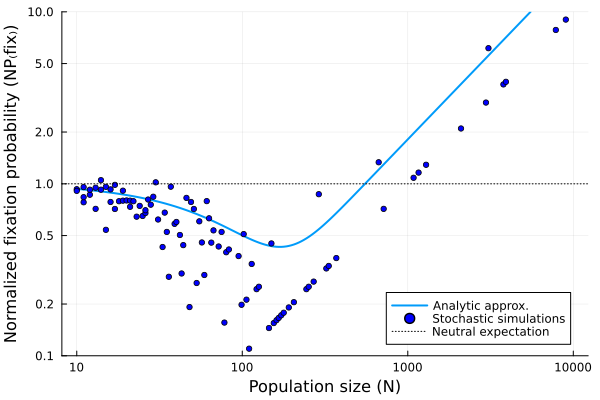
\includegraphics[scale=0.5]{./imgs/fig1J6.png}

    With the 2-locus model: \\
    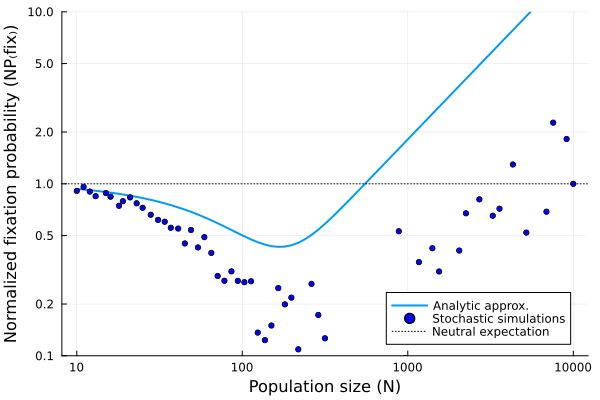
\includegraphics[scale=0.5]{./imgs/fig1J_2locus.png}

    As you can see from the graphs, there does not appear to be any significant difference between the 100- and 2-locus models, other than possibly that the 100-locus model fits the analytic approximation better. However, the 2-locus model is still clearly able to demonstrate the U-shaped curve demonstrating sign-inversion behavior like in the 100-locus model.
  \end{mysolution}

  \item  Notice the assumption in the caption to figure 1: ”Mutators mutate 100 times faster than
  nonmutators.” Do results change if mutators only mutate 10 times faster? Does the choice of
  100 matter?
  \par\begin{mysolution}
    With the 2-loci model, mutation factor = 10: \\
    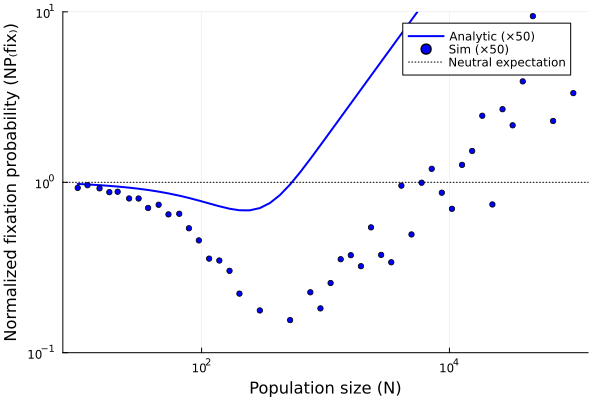
\includegraphics[scale=0.5]{./imgs/fig1J_2lociTest10.png}

    Testing mutation factor in the 2-loci model over a range of mutator factor values (1-100): \\
    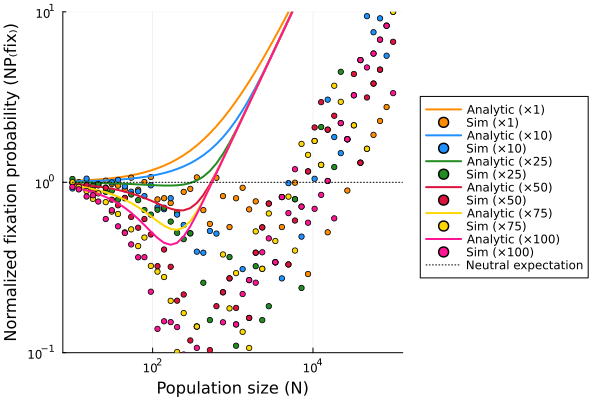
\includegraphics[scale=0.5]{./imgs/fig1J6_test3.png}


    The plot shows how the normalized fixation probability $NP_{fix}$ of mutator alleles varies with population size $N$ and mutator strength (mutation rate increase factor). The orange curves (representing x1, i.e., non-mutators) lie near the neutral expectation line especially for lower population sizes, as expected for non-mutators. As mutator strength increases, a nonlinear, U-shaped trend emerges: fixation probability dips below neutrality at intermediate $N$ due to deleterious load, then rises above neutrality at large $N$ due to beneficial hitchhiking.
    
    When the mutator strength is set to 10 (blue curve), the fixation probability is still U-shaped but less pronounced than for higher mutation rates. This indicates that while the nonlinear trend remains, it is less sensitive to population size at lower mutation rates. The sign inversion becomes sharper and shifts leftward with increasing mutator strength. This confirms the prediction from Raynes et al. (2018) that strong mutators can be selectively favored in large populations despite their deleterious burden.
  \end{mysolution}
\end{enumerate}

\titledquestion{Problem 2} [20] 
Species living at the edge of their natural range can fail to adapt to local conditions because
of the constant inflow of migrants from the center of the range. Consider a haploid model
of selection where selection in a marginal patch favors allele $a$: $W_A = (1-s)$ and $W_a = 1$.
Adults migrate into the marginal patch from a more favorable area at rate $m$. We will assume
that these migrants all carry allele $A$, which is favored in the core habitat (see Figure). After
migration, the frequency of the locally unfit allele A becomes $p(t + 1) = (1 - m)p' + m$, where
$p'$ is the frequency of allele $A$ in the local population after selection but before migration:
$p' = \frac{p(t)(1-s)}{p(t)(1-s)+(1-p(t))}$ .

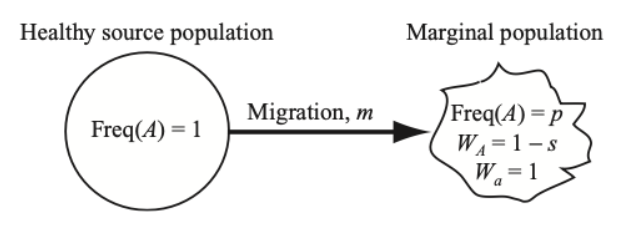
\includegraphics[scale=0.5]{fig.png}

\begin{enumerate}
  \item Find the two equilibria of this model.
  
  \par\begin{mysolution}
    After selection but before migration, we have
    \[
    p' = \frac{p(1-s)}{p(1-s)+(1-p)} = \frac{p(1-s)}{1-sp}
    \]
    After migration we get 
    \[
    p_{t+1} = (1-m)p' + m
    \]
    Substituting p' into the post-migration equation, we have
    \[
    p_{t+1} = (1-m) \frac{p(1-s)}{1-sp} + m
    \]
    At equilibrium, $p_{t+1} = p$, so we have
    \begin{align}
    p &= (1-m) \frac{p(1-s)}{1-sp} + m \\
    p(1-sp) &= (1-m) p(1-s) + m(1-sp) \\
    p - p^2s &= (1-m)p(1-s) + m(1-sp) \\
    p - p^2s &= (1-m)p(1-s) + m - msp \\
    p - p^2s - (1-m)p(1-s) - m + msp &= 0 \\
    p (m + s - ms) - sp^2 + msp - m &= 0 \\
    p(m + s - ms) - sp^2(1-m) - m &= 0 \\
    -sp^2 (1 - m) + p(m + s - ms) - m &= 0
    \end{align}
    This is quadratic in $p$, so using the quadratic formula the two equilibria are as follows:
    \[
    p^* = \frac{-(m + s - ms) \pm \sqrt{(m+s-ms)^{2} - 4(-s(1-m))(-m)}}{2(-s(1-m))}
    \]
  \end{mysolution}
  \item What conditions must hold for polymorphic equilibrium to be biologically valid?
  \par\begin{mysolution}
    For the polymorphic equilibrium to be biologically valid, we need both equilibria to lie in the interval [0, 1]. This means that the discriminant of the quadratic must be non-negative, such that $(m+s-ms)^{2} - 4(-s(1-m))(-m) \geq 0$. Secondly, the two roots/equilibria described above must be within the interval [0, 1]. And thirdly, the parameters must satisfy $m<s$ to ensure that selection favors allele $a$ over $A$ in the marginal patch. This ensures that the fitness of allele $a$ is higher than that of $A$ in the marginal patch so that the rare, locally beneficial allele aa can increase despite the influx of maladapted migrants, allowing both alleles to persist in the population.
  \end{mysolution}
  
  \item Determine when allele a will disappear from the population when rare despite the fact that it is locally favored by examining the stability of the equilibrium at peq = 1.
  \begin{mysolution}
    To determine when allele $a$ will disappear from the population when rare, we need to examine the stability of the equilibrium at $p = 1$, when maladapted migrant allele $A$ fixates in the population. 

    Using the update equation derived in part 1 we have
    \[
    p' = \frac{p(1-s)}{1-sp}
    \]
    and then given the recursion relation
    \[
    p(t+1) = (1-m)p' + m
    \]
    Substituting $p = 1$ into the equation for $p'$ gives
    \[
    f(p) = p(t+1) = (1-m) \frac{p(1-s)}{1-sp} + m
    \]

    Computing the derivative of the recursion relation at $p = 1$ will help us determine the stability of the equilibrium. We can find the derivative of $p_{t+1}$ with respect to $p$ at $p=1$ as follows:
    \[
    f(p) = (1-m) \frac{p(1-s)}{1-sp} + m
    \]
    \begin{align*}
    \frac{df}{dp} &= (1-m) \left( \frac{(1-s)(1-sp) + p(1-s)(-s)}{(1-sp)^2} \right) \\
    &= (1-m) \left( \frac{(1-s)(1-sp) + ps(1-s)}{(1-sp)^2} \right) \\
    &= (1-m) \left( \frac{(1-s)(1 - sp + ps)}{(1-sp)^2} \right) \\
    &= (1-m) \frac{(1-s)(1)}{(1-sp)^2} \\
    f'(p) &= \frac{(1-m)(1-s)}{(1-sp)^2}
    \end{align*}

    Evaluating the derivative at $p = 1$ we have
    \[
    f'(1) = \frac{(1-m)(1-s)}{(1-s)^2} = \frac{1-m}{1-s}
    \]

    So the equilibrium at $p = 1$ is stable if $|f'(1)| < 1$, which implies
    \[
    \frac{|1-m|}{|1-s|} < 1
    \]
    Since all parameters $\in [0,1]$, we can analyze the inequality as follows:
    \[
    \frac{1-m}{1-s} < 1 \implies 1-m < 1-s \implies s < m
    \]

    Thus, the equilibrium at $p=1$ (fixation of maladapted allele $A$) is stable when 
    \(
    m>s
    \)
    In this case, allele $a$ disappears from the population when rare, despite being locally favored. This is because the influx of maladapted migrant allele $A$ from the core habitat overwhelms local selection towards allele $a$ in the marginal patch, preventing the rare beneficial allele from increasing in frequency.
\end{mysolution}
\end{enumerate}

\titledquestion{Problem 3} [30] 

The goal of this problem is to learn how to incorporate recombination in your equations and
simulations. Consider this followup paper to the Salathe paper, incorporating recombination
in their equations: https://pubmed.ncbi.nlm.nih.gov/21212229/ (Liberman et al 2011)
Modify your code from the last homework, the one attempting to replicate the Salathe results
and now incorporate non-zero recombination. Discuss what you observe. You get to choose
what plot to make and what parameters to plot, but please upload your code.

\par\begin{mysolution}
    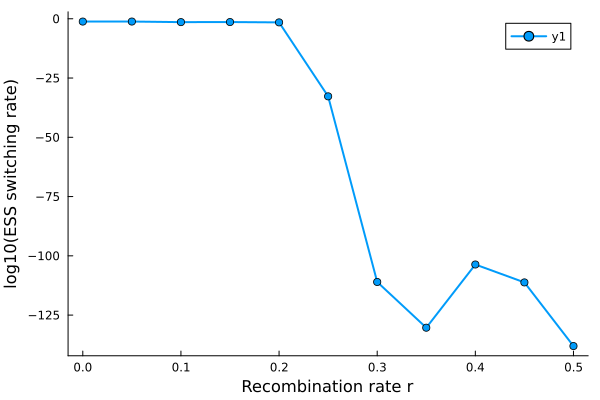
\includegraphics[scale=0.5]{./imgs/essRecombLiberman.png} 

    Figure 1. Fixation probability of mutator alleles with varying recombination rates.

    Figure 1 shows how the ESS depends on the recombination rate $r$ when environmental variance is held constant at 20 and selection strength is moderate ($s=0.1$). For low recombination rates ($r \leq 0.2$), the ESS switching rate remains relatively high and stable, consistent wit the optimal switching rate predicted by $\frac{1}{n}$, where $n=20$. However, as $r$ increases beyond $0.2$, the ESS rapidly declines, eventually dropping to extremely low values suggesting that high recombination essentially eliminates switching. This pattern supports the finding from Liberman et al. (2011) that recombination disrupts the genetic linkage between modifier alleles and the phenotypes they influence, thereby preventing the maintenance of adaptive switching through natural selection.

    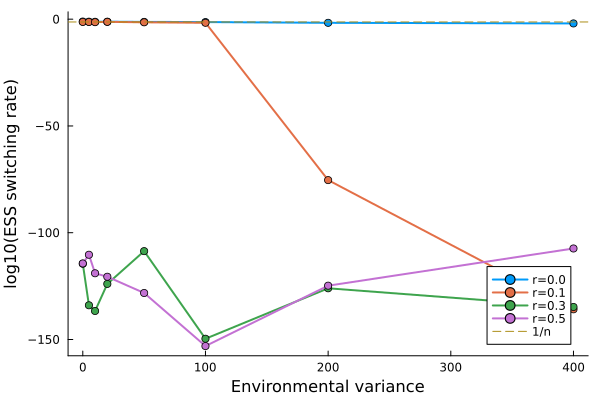
\includegraphics[scale=0.5]{./imgs/essVarRecomb.png}

    Figure 2. Fixation probability of mutator alleles as a function of variance in environmental switching. 

    Figure 2 plots the ESS switching rate as a function of environmental variance for four different recombination rates ($r \in \{0.0, 0.1, 0.3, 0.5\}$), while keeping selection constant at $s=0.1$. When $r=0.0$, the ESS remains close to the predicted value of $\frac{1}{n}$ (where $n=20$) across all variances, mirroring the original results of Salathe et al. for symmetric fitness landscapes. However, as recombination increases, ESS becomes increasingly sensitive to environmental unpredictability, where at $r=0.3$ and $r=0.5$, even small increases in variance lead to dramatic drops in switching rates. THis demonstrates that recombination exacerbates the negative effects of environmental variance on switching, as it breaks down the tight genetic linkage between the mutator and the adaptive phenotypes they influence. Thus, it makes it nearly impossible for stochastic switching to evolve in unpredictable environments when recombination is present.
\end{mysolution}

\titledquestion{Problem 4} [20] 

“Memes” are cultural traits, such as inventions and fads, whose spread within a population
can be modeled. Consider a meme that is adopted slowly, only after an individual sees two
other individuals with the meme. A recursion equation for the fraction of the population with
the meme f might be $f (t + 1) = f (t)(1 - \gamma) + \alpha f (t)2(1 -f(t))$, where $\gamma$ represents the loss of the meme and the fraction of individuals that adopt the meme is $\alpha$ per time step (squared reflects our assumption that the meme spreads only after witnessing two individuals with the
meme).

\begin{enumerate}
  \item Find the three equilibria of this model
  \par\begin{mysolution}
    Given the function
    \[
    f(t+1) = f(t) (1-\gamma) + \alpha f(t)^2 (1-f(t))
    \]
    We want to solve for the equilibria by setting $f(t+1) = f(t) = f^*$, where $f^*$ is the equilibrium frequency of the meme. Thus, we have
    \[
    f^* = f^*(1-\gamma) + \alpha f^{*2} (1-f^{*})
    \]
    Rearranging and simplifying, we have
    \begin{align*}
      f^* - f^*(1-\gamma) - \alpha f^{*2}(1-f^*) &= 0 \\
      f^*\gamma - \alpha f^{*2}(1-f^*) &= 0 \\
      f^*(\gamma - \alpha f^*(1-f^*)) &= 0
    \end{align*}
    This gives us a solution at $f^* = 0$ (the trivial equilibrium where no one has the meme). Additionally, we have non-zero solutions when we solve
    \[
    \gamma = \alpha f^*(1-f^*)
    \]
    which is quadratic in $f^*$, leading to 
    \[
    \alpha f^{*2} - \alpha f^* + \gamma = 0
    \]
    Solving for $f^*$ using the quadratic formula we have
    \[
    f^* = \frac{\alpha \pm \sqrt{\alpha^2 - 4\alpha\gamma}}{2\alpha} = \frac{1 \pm \sqrt{1- \frac{4\gamma}{\alpha}}}{2}
    \]
    Thus, the three equilibria are
    \[
    f^* = 0 
    \]
    \[
    f^* = \frac{1-\sqrt{1-\frac{4\gamma}{\alpha}}}{2} 
    \]
    \[
    f^* = \frac{1+\sqrt{1-\frac{4\gamma}{\alpha}}}{2}
    \]

  \end{mysolution}

  \item Plot the recursion $f(t +1)$ versus $f(t)$ for $\gamma = 0.4$ and $\alpha = 2$ along with the diagonal line. Mark each equilibrium with an X
  \par\begin{mysolution}
    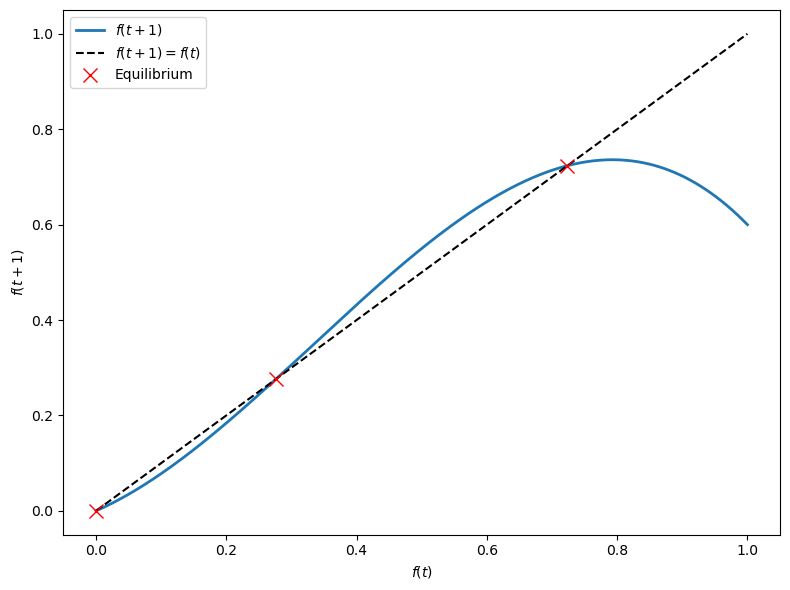
\includegraphics[scale=0.5]{./imgs/memes.png}
  \end{mysolution}

  \item From the slope of the recursion equation at each equilibrium (on the graph), specify which equilibria are stable ($S$) and which are unstable ($U$).
  \par\begin{mysolution}
    At the equilibrium at $f^* = 0$, the slope of the curve is much lower than that of the identity line (1), suggesting that the equilibrium at $f^* = 0$ is stable ($S$). For the middle equilibrium at approximately $f^* \approx 0.3$, the slope of the recursion is greater than 1, indicating that this equilibrium is unstable ($U$). Finally, for the upper equilibrium at approximately $f^* \approx 0.75$, the slope of the recursion is less than 1, indicating that this equilibrium is stable ($S$).
  \end{mysolution}
\end{enumerate}



\end{questions}
\end{document}
